\section{Convolutional Codes}
\subsection{TCM - Trellis Coded Modulation}
\subsubsection{Convolutional Coding - Faltungs Code}
Ein Faltungs Code besitzt zur Logikschaltung zus\"atzlich noch Memory, so dass
nicht nur der aktuelle Eingang sondern auch noch $n$-vorherige Eing\"ange zum
Ausgang verrechnet werden. Es gibt m unterschiedliche Ausg\"ange. 
Je nach Vorgeschichte, k\"onnen nur noch ganz bestimmte Kombinationen auftreten,
was dann die Decodierung besser macht.\\
\begin{minipage}{9cm}
	Beispiel mit k=1; n=2; m=2 $\to$ 1/2 codierung\\
	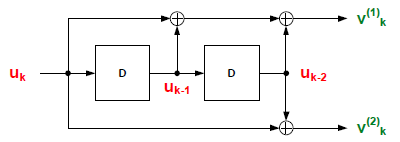
\includegraphics[width=9cm]{./bilder/covolutionSchemata.png}
\end{minipage}
\hspace{5mm}
\begin{minipage}{8cm}
\vspace{4mm}
	mit dazugeh\"origem Encoder State Diagram\\
\hspace{5mm}
	\includegraphics[width=6cm]{./bilder/covolutionStateDiagram.png}
\end{minipage}

\subsubsection{Decodierung}
Eine gute Variante die FaltungsCodes zu dekodieren ist dies mit einem Trellis
Diagram zu machen: \\
\begin{minipage}{10cm}
	\begin{liste}
		\item Zuerst Punkte entsprechend der m\"oglichen Speicherinhalte einzeichnen.
		\item M\"ogliche Verbindungen einzeichnen.
		\item Sollwerte einzeichnen (z.B. 0/00).
		\item Fehler zu den einzelnen Punkten eintragen (ev. die Euklidische Distanz).
		\item Wenn zwei Wege zu einem Punkt kommen, den h\"oherwertigen Weg streichen.
		\item Am Schluss den Weg nehmen der den kleinsten Fehler ergibt.
	\end{liste}
\end{minipage}
\begin{minipage}{9cm}
	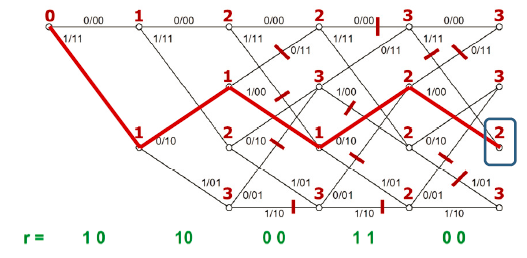
\includegraphics[width=9cm]{./bilder/Trelli.png}
\end{minipage}

\subsubsection{Euklidische Distanz}
\begin{minipage}{13cm}
	Die \textbf{euklidische Distanz} ist der Abstand zwischen zwei
	unterschiedlichen Modulationspositionen.\\
	Die \textbf{freie euklidische Distanz} ist der minimale Abstand zwischen zwei
	unterschiedlichen Modulationspositionen in der ganzen Modulation.\\
	$d^2_{free}=\min \limits_{a_k \neq a_{k}^{'}} \sum \limits_k
	d^2(a_k,a_{k}^{'})$\\
	zB.	$d^2_{min}=1 + 1 -2\cos (\alpha)= 2-\sqrt{2} = 0.586$\\
	Der \textbf{Coding Gain} ist um welchen Faktor der SNR schlechter sein darf.\\
	$G = \frac{d^2_{free,coded}}{d^2_{min, uncoded}}$
\end{minipage}
\begin{minipage}{6cm}
	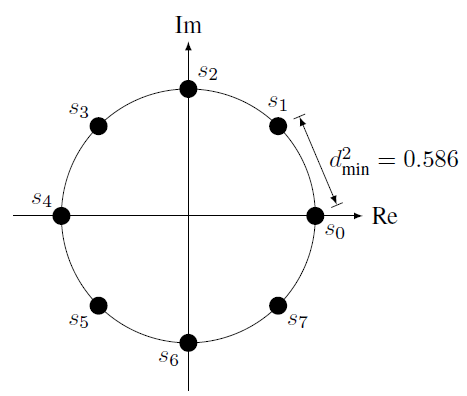
\includegraphics[width=6cm]{./bilder/EuklidischeDistanz.png}
\end{minipage}